\subsection{Anforderungsspezifikation}
In dieser Sektion werden die Ergebnisse der Anforderungsanalyse in Form von diversen Diagrammen und Tabellen festgehalten. Ziel ist es, nötige Einschränkungen für das System zu definieren während genug Spielraum für die Umsetzung gelassen wird. 

\subsubsection{Funktionale Anforderungen}\label{sec:functional-requirements}
Aufgrund der Fortsetzung der Arbeit existieren im Bezug auf die Anforderungen Überlappungen bei allen Use Cases, die für den wesentlichen Ablauf der Applikation nötig sind. Im Folgenden werden die Gemeinsamkeiten und Unterschiede beschrieben und detailliert auf Neuigkeiten eingegangen. 


\begin{figure}[h]
	\centering
	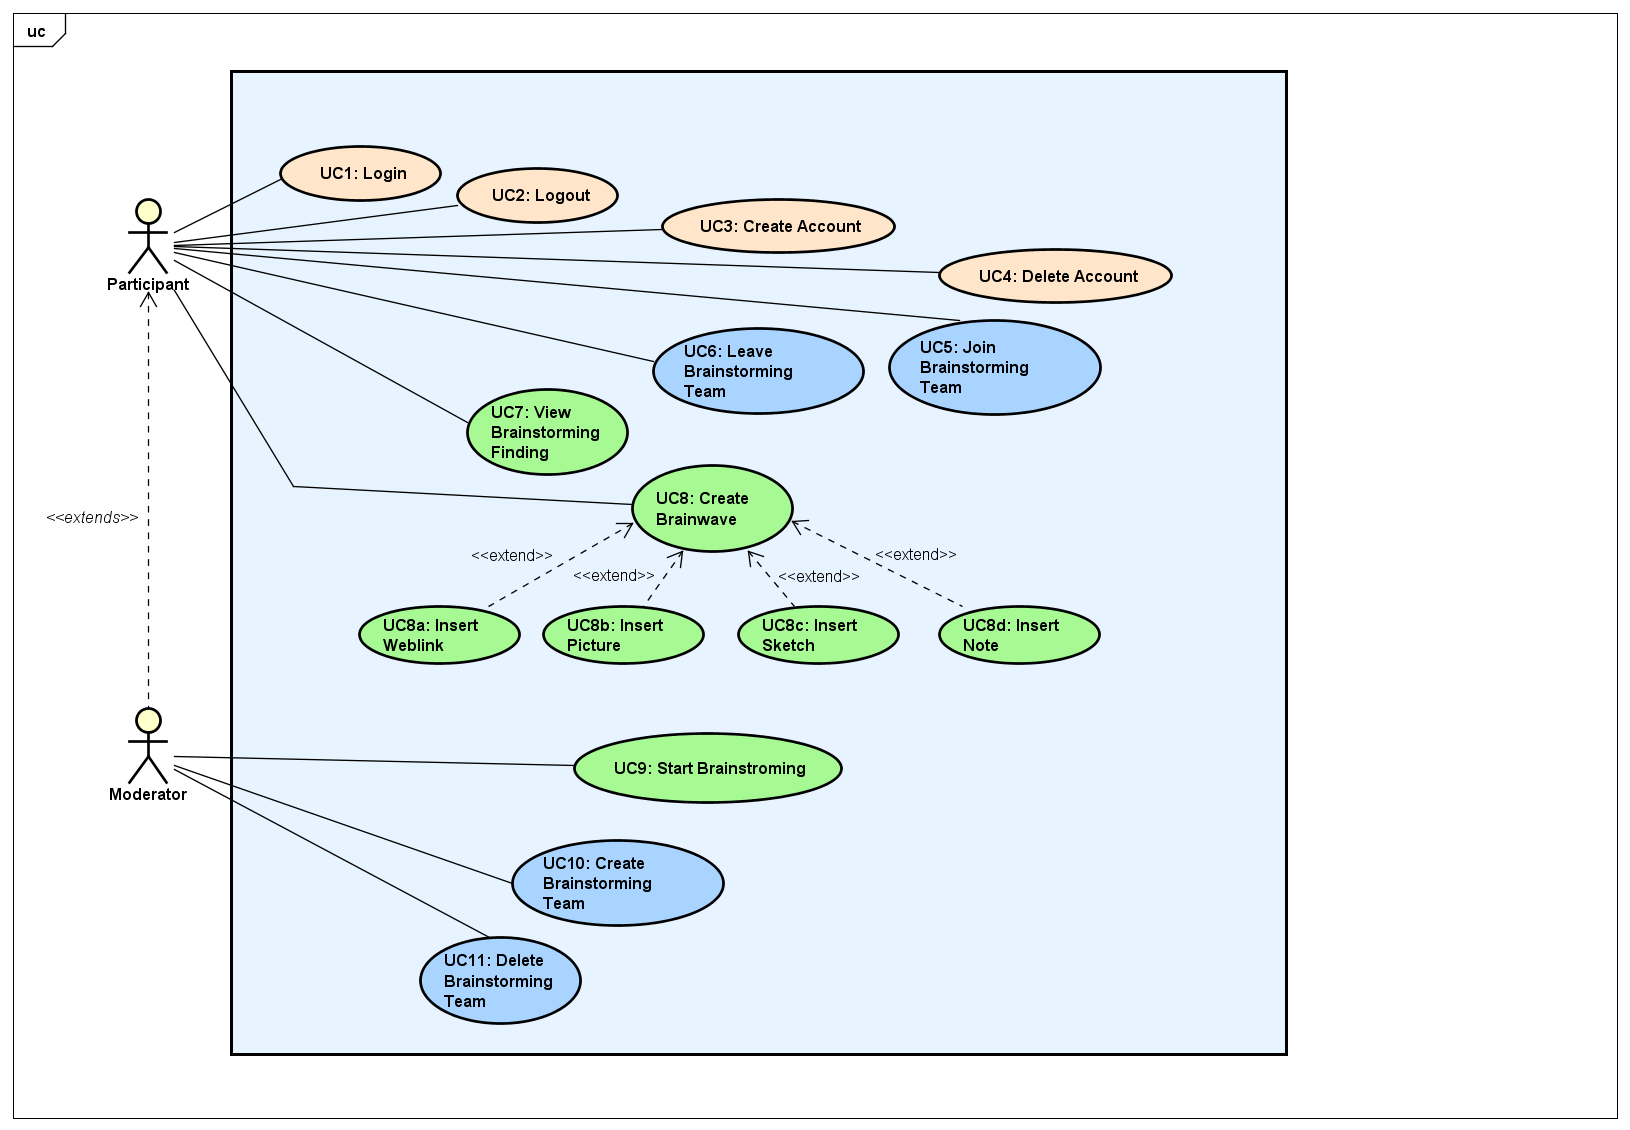
\includegraphics[width=1\linewidth]{./img/anforderungen/UC-Methode635.png}
	\caption{Use-Case Diagramm Methode 635}
	\label{fig:uc-methode635}
\end{figure}
Abbildung \ref{fig:uc-methode635} zeigt das Use-Case Diagramm für diese Arbeit. Es gibt einige Abweichungen zur Studienarbeit. Im Diagramm sind 8 Use-Cases in blasser Farbe gestaltet, bei diesen handelt es sich um bereits implementierte Features im Umfang der Studienarbeit. 

Wichtig zu erwähnen ist dabei, dass UC12: Create Brainstorming Finding erst im Nachhinein hinzugekommen ist. Dies ist so, weil zu Beginn der Entwicklung wir die Annahme trafen, dass für jedes Team genau ein Brainstorming entsteht und zwar zum Zeitpunkt des Starts des Brainstorming Findings (UC9). Wie wir aber im Verlaufe der Zeit feststellten, war die Umsetzung mit mehreren Brainstorming Findings pro Team innert vertretbarer Zeit möglich. So entstand ein zusätzlicher Use-Case, der nicht mehr implizit mit UC9: Start Brainstorming Finding ausgeführt wurde.

Weiter sind Use-Cases in satter Farbe erkennbar. Bei diesen handelt es sich um diejenigen, welche in dieser Arbeit im Fokus liegen. Komplett neu hinzugekommen sind UC8e: Insert Pattern, UC8f: Insert Video und UC13: Export BrainstormingFinding. Als zentraler Use-Case wird zudem UC8c: Draw Sketch angesehen. Im folgenden Kapitel werden nun die in dieser Arbeit relevanten Use-Cases kurz beschrieben. Im Kapitel \ref{par:fully-dressed-uc} sind alle zu implementierenden Sub-Use-Cases von UC8: Create Brainwave im fully-dressed Stil detailliert erläutert.
\paragraph{Brief Use-Cases}~\\
Die für diese Arbeit relevanten Use-Cases sind hier beschrieben.

\begin{basedescript}{
		\desclabelstyle{\multilinelabel}
		\desclabelwidth{4.5cm}
		\setlength{\itemsep}{5ex}}
	
	\item[\textit{UC2: }Logout] Als eingeloggter Participant will ich mich ausloggen, sodass das Startfenster wieder erscheint.
	
	\item[\textit{UC6: }Leave Brainstorming Team] Als Participant will ich ein beigetretenes Team verlassen können.
		
	\item[\textit{UC8: }Create Brainwave] Als Participant will ich während einer Brainstorming Session ein Brainwave (bestehend aus mehreren Ideen) erstellen und einreichen können. 
	
	\item[\textit{UC8a: }Insert Weblink] Als Participant will ich einen Weblink in mein aktuelles Sheet einfügen können.
	
	\item[\textit{UC8b: }Integrate Picture] Als Participant will ich ein Bild in mein aktuelles Sheet integrieren können.
	
	\item[\textit{UC8c: }Draw Sketch] Als Participant will ich in mein aktuelles Sheet zeichnen können.
	
	\item[\textit{UC8e: }Insert Pattern] Als Participant will ich aus Vorlagen software-relevante Patterns in mein aktuelles Sheet einfügen können.
	
	\item[\textit{UC8f: }Record Video] Als Participant will ich ein Video aufnehmen und in mein aktuelles Sheet einfügen können.
	
	\item[\textit{UC11: }Delete Brainstorming Team] Als Moderator will ich ein Brainstorming Team löschen können.
	
	\item[\textit{UC13: }Export Brainstorming Finding] Als Participant will ich ein abgeschlossenes \textit{BrainstormingFinding }exportieren können. 
\end{basedescript}
\vspace{1cm}

\paragraph{Fully-Dressed Use-Cases}
\label{par:fully-dressed-uc}~\\
Die fully-dressed Use-Cases folgen den im Modul \textit{Software Engineering 1} des Bachelorstudiums Informatik der HSR empfohlenen Punkten.
\renewcommand{\arraystretch}{1.35}
\begin{center}
	\begin{longtable}{| c | p{7cm} |}
		\hline
		\multicolumn{2}{|c|}{\textbf{Use-Case 8a: Insert Weblink}}\\
		\hline\hline
		\textit{Primary Actor} & Participant\\
		\hline
		\textit{Stakeholders \& Interests} & Ein Participant wünscht als Teil seiner Brainwave einen Weblink zu teilen. \\
		\hline
		\textit{Preconditions} & Participant existiert im System (UC3), ist eingeloggt (UC1) und einer Gruppe beigetreten (UC5). Des weiteren existiert mindestens ein BrainstormingFinding (UC12), welches schon gestartet ist (UC9).\\
		\hline
		\textit{Post Conditions/Success Guarantee} & Der Weblink ist erfolgreich in der Brainwave gespeichert und kann in einer nächsten Runde von den anderen Participants angesehen werden.\\
		\hline
		\textit{Main Success Scenario/Basic Flow} & 
		\begin{enumerate}[noitemsep]
			\item Der Participant speichert sich den gewünschten Weblink in den Zwischenspeicher des Smartphones.
			\item Der Participant fügt mittels Einfügen den Text in das Textfeld ein.
			\item Der Participant speichert den Link mittels commit in seiner Brainwave ab.
		\end{enumerate}\\
		\hline
		\textit{Alternative Flows} &
		-\\
		\hline
		\textit{Frequency of Occurrence} & gelegentlich, erweiterte Kernfunktionalität.\\
		\hline
	\end{longtable}
\end{center}

\renewcommand{\arraystretch}{1.35}
\begin{center}
	\begin{longtable}{| c | p{7cm} |}
		\hline
		\multicolumn{2}{|c|}{\textbf{Use-Case 8b: Integrate Picture}}\\
		\hline\hline
		\textit{Primary Actor} & Participant\\
		\hline
		\textit{Stakeholders \& Interests} & Ein Participant wünscht als Teil seiner Brainwave einen Bild zu teilen. \\
		\hline
		\textit{Preconditions} & Participant existiert im System (UC3), ist eingeloggt (UC1) und einer Gruppe beigetreten (UC5). Des weiteren existiert mindestens ein BrainstormingFinding (UC12), welches schon gestartet ist (U9).\\
		\hline
		\textit{Post Conditions/Success Guarantee} & Das Bild ist erfolgreich in der Brainwave gespeichert und kann in einer nächsten Runde von den anderen Participants angesehen werden.\\
		\hline
		\textit{Main Success Scenario/Basic Flow} & 
		\begin{enumerate}[noitemsep]
			\item Der Participant klickt den Plus-Button (o.Ä) neben dem Text-Eingabefeld.
			\item Das System zeigt ein Menü mit weiteren Ideentypen (unter anderem das Bild) an.
			\item Der Participant klickt auf den Menüeintrag, um ein Bild aufzunehmen.
			\item Das Smartphone öffnet die Kamerafunktion.
			\item Der Participant macht ein Foto und speichert das Bild mit dem entsprechenden Button in seine Brainwave. 
		\end{enumerate}\\
		\hline
		\textit{Alternative Flows} &
		- \\
		\hline
		\textit{Frequency of Occurrence} & gelegentlich, erweiterte Kernfunktionalität.\\
		\hline
	\end{longtable}
\end{center}

\renewcommand{\arraystretch}{1.35}
\begin{center}
	\begin{longtable}{| c | p{7cm} |}
		\hline
		\multicolumn{2}{|c|}{\textbf{Use-Case 8c: Draw Sketch}}\\
		\hline\hline
		\textit{Primary Actor} & Participant\\
		\hline
		\textit{Stakeholders \& Interests} & Ein Participant wünscht als Teil seiner Brainwave eine eigene Skizze zu zeichnen. \\
		\hline
		\textit{Preconditions} & Participant existiert im System (UC3), ist eingeloggt (UC1) und einer Gruppe beigetreten (UC5). Des weiteren existiert mindestens ein BrainstormingFinding (UC12), welches schon gestartet ist (U9).\\
		\hline
		\textit{Post Conditions/Success Guarantee} & Die gezeichnete Skizze ist erfolgreich in der Brainwave gespeichert und kann in einer nächsten Runde von den anderen Participants angesehen (aber nicht bearbeitet) werden.\\
		\hline
		\textit{Main Success Scenario/Basic Flow} & 
		\begin{enumerate}[noitemsep]
			\item Der Participant klickt den Plus-Button (o.Ä) neben dem Text-Eingabefeld.
			\item Das System zeigt ein Menü mit weiteren Ideentypen (unter anderem die Skizze) an.
			\item Der Participant klickt auf den Menüeintrag, um eine Skizze zu zeichnen.
			\item Das Smartphone öffnet im App selbst eine entsprechende View, um Bilder zu zeichnen.
			\item Ist der Participant zufrieden mit der Skizze, speichert diese mit dem entsprechenden Button in seine Brainwave.
		\end{enumerate}\\
		\hline
		\textit{Alternative Flows} &
		-\\
		\hline
		\textit{Frequency of Occurrence} & gelegentlich, erweiterte Kernfunktionalität.\\
		\hline
	\end{longtable}
\end{center}

\renewcommand{\arraystretch}{1.35}
\begin{center}
	\begin{longtable}{| c | p{7cm} |}
		\hline
		\multicolumn{2}{|c|}{\textbf{Use-Case 8e: Insert Pattern}}\\
		\hline\hline
		\textit{Primary Actor} & Participant\\
		\hline
		\textit{Stakeholders \& Interests} & Ein Participant wünscht als Teil seiner Brainwave einen bekanntes Pattern zu teilen. \\
		\hline
		\textit{Preconditions} & Participant existiert im System (UC3), ist eingeloggt (UC1) und einer Gruppe beigetreten (UC5). Des weiteren existiert mindestens ein BrainstormingFinding (UC12), welches schon gestartet ist (U9) und vom Typ SoftwareLösung ist.\\
		\hline
		\textit{Post Conditions/Success Guarantee} & Das Microservice-API-Pattern (Symbol und Name von MAP\cite{microservices-api}) ist erfolgreich in der Brainwave gespeichert und kann in einer nächsten Runde von den anderen Participants angesehen und auf einer externen Webseite genauer begutachtet werden.\\
		\hline
		\textit{Main Success Scenario/Basic Flow} & 
		\begin{enumerate}[noitemsep]
			\item Der Participant klickt den Plus-Button (o.Ä) neben dem Text-Eingabefeld.
			\item Das System zeigt ein Menü mit weiteren Ideentypen (unter anderem das Pattern) an.
			\item Der Participant klickt auf den Menüeintrag, um eine Auswahl von verschiedenen Patterns zu erhalten.
			\item Er wählt das passende Microservice-API-Pattern aus und speichert dieses mit dem entsprechenden Button in seine Brainwave.
		\end{enumerate}\\
		\hline
		\textit{Alternative Flows} &
		-\\
		\hline
		\textit{Frequency of Occurrence} & gelegentlich, erweiterte Kernfunktionalität.\\
		\hline
	\end{longtable}
\end{center}

\renewcommand{\arraystretch}{1.35}
\begin{center}
	\begin{longtable}{| c | p{7cm} |}
		\hline
		\multicolumn{2}{|c|}{\textbf{Use-Case 8b: Record Video}}\\
		\hline\hline
		\textit{Primary Actor} & Participant\\
		\hline
		\textit{Stakeholders \& Interests} & Ein Participant wünscht als Teil seiner Brainwave ein Video aufzunehmen. \\
		\hline
		\textit{Preconditions} & Participant existiert im System (UC3), ist eingeloggt (UC1) und einer Gruppe beigetreten (UC5). Des weiteren existiert mindestens ein BrainstormingFinding (UC12), welches schon gestartet ist (U9). Die Länge des Videos wird auf wenige Sekunden limitiert, da dieses sonst länger werden kann als die zur Verfügung stehende Zeit.\\
		\hline
		\textit{Post Conditions/Success Guarantee} & Das Video ist erfolgreich in der Brainwave gespeichert und kann in einer nächsten Runde von den anderen Participants angesehen werden.\\
		\hline
		\textit{Main Success Scenario/Basic Flow} & 
		\begin{enumerate}[noitemsep]
			\item Der Participant klickt den Plus-Button (o.Ä) neben dem Text-Eingabefeld.
			\item Das System zeigt ein Menü mit weiteren Ideentypen (unter anderem das Video) an.
			\item Der Participant klickt auf den Menüeintrag, um ein Video aufzunehmen.
			\item Das Smartphone öffnet die Kamerafunktion.
			\item Der Participant macht ein kurzes Video und speichert dieses mit dem entsprechenden Button in seine Brainwave.
		\end{enumerate}\\
		\hline
		\textit{Alternative Flows} &
		-\\
		\hline
		\textit{Frequency of Occurrence} & selten, erweiterte Kernfunktionalität.\\
		\hline
	\end{longtable}
\end{center}

\renewcommand{\arraystretch}{1.35}
\begin{center}
	\begin{longtable}{| c | p{7cm} |}
		\hline
		\multicolumn{2}{|c|}{\textbf{Use-Case 13: Export BrainstormingFinding}}\\
		\hline\hline
		\textit{Primary Actor} & Participant\\
		\hline
		\textit{Stakeholders \& Interests} & Ein Participant wünscht die ausgearbeiteten Ideen zu exportieren. \\
		\hline
		\textit{Preconditions} & Participant existiert im System (UC3), ist eingeloggt (UC1) und einer Gruppe beigetreten (UC5). Des weiteren existiert mindestens ein BrainstormingFinding (UC12), welches schon abgeschlossen ist.\\
		\hline
		\textit{Post Conditions/Success Guarantee} & Alle Ideen des ausgewählten BrainstormingFinding werden in einem passenden Format exportiert (vorstellbar wäre Markdown), sodass diese für andere Tätigkeiten weitergenutzt werden können.\\
		\hline
		\textit{Main Success Scenario/Basic Flow} & 
		\begin{enumerate}[noitemsep]
			\item Der Participant navigiert zum gewünschten BrainstormingFinding, welches er exportieren möchte.
			\item Er klickt auf den Button export (o.Ä).
			\item Das System exportiert alle eingereichten Ideen an einen Ort nach Wahl.
		\end{enumerate}\\
		\hline
		\textit{Alternative Flows} &
		-\\
		\hline
		\textit{Frequency of Occurrence} & gelegentlich, erweiterte Kernfunktionalität.\\
		\hline
	\end{longtable}
\end{center}

\paragraph{Sequenzdiagramm}~\\
\label{par:sequence-diagramm}
Der Vollständigkeits halber haben wir in Abbildung \ref{fig:Seq-Methode635} nochmals das erarbeitete Sequenzdiagramm unserer Studienarbeit \cite{methode635-sa} dargestellt. Darin ist der Prozess vom Erstellen des BrainstormingTeams bis zum Abschliessen der Brainwave modelliert. 


\begin{landscape}
	\label{subsec:timeline}
		\begin{figure}[h]
		\centering
			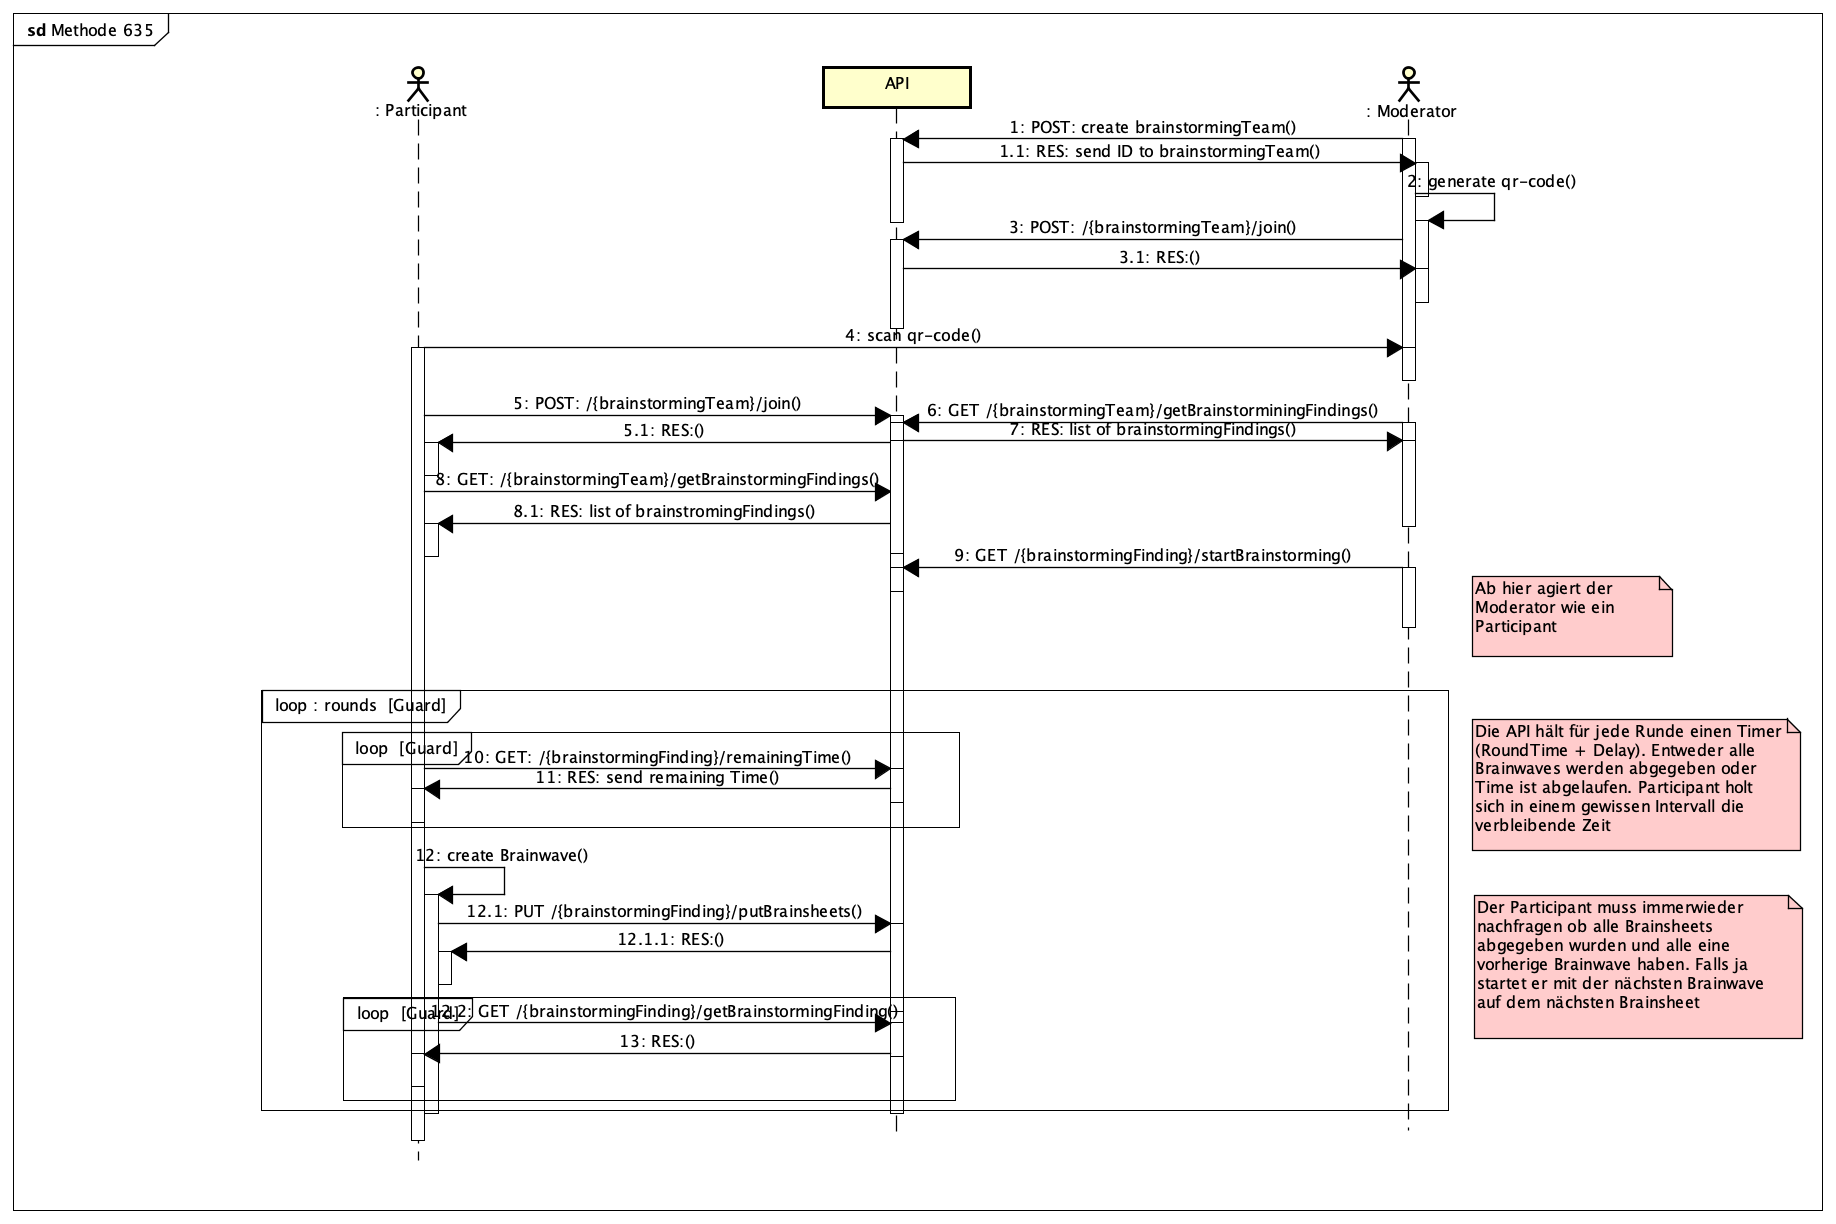
\includegraphics[width=1\linewidth]{img/anforderungen/Seq-Methode635}
		\caption[Ablauf der Kernlogik]{Ablauf der Kernlogik}
		\label{fig:Seq-Methode635}
		\end{figure}
	\vspace{0.5cm}
\end{landscape}


Zusätzlich dazu haben wir in Abbildung \ref{fig:Seq-Draw-Sketch} und \ref{fig:Seq-Insert-Pattern}, die aus unserer Sicht wichtigsten neuen Use-Cases (UC8c und UC8e) als Ablaufdiagramm gezeichnet und beschreiben, wo diese im Ablauf zum Tragen kommen.

\begin{basedescript}{
		\desclabelstyle{\multilinelabel}
		\desclabelwidth{4.5cm}
		\setlength{\itemsep}{5ex}}
	
	\item[\textit{UC8c Draw Sketch:}] Nachdem eine Brainwave gestartet ist (siehe 12 in Abbildung \ref{fig:Seq-Methode635}) und sich der Participant dazu entschlossen hat, eine Skizze zu zeichnen und damit zufrieden ist, speichert er diese in seine Brainwave. Dabei wird ein POST-Request an das API gesendet, welcher das gezeichnete Bild in der Datenbank speichert. Als Antwort wird eine ID an den Participant bzw. an die Applikation zurück geschickt.
	In einem nächsten Schritt wird wie bis anhin (siehe 12.1 in Abbildung \ref{fig:Seq-Methode635}) das gesamte Brainsheet, welches nun auch die ID in der entsprechenden SketchIdee gespeichert hat, an die API geschickt.
\end{basedescript}

\begin{figure}[h]
	\centering
	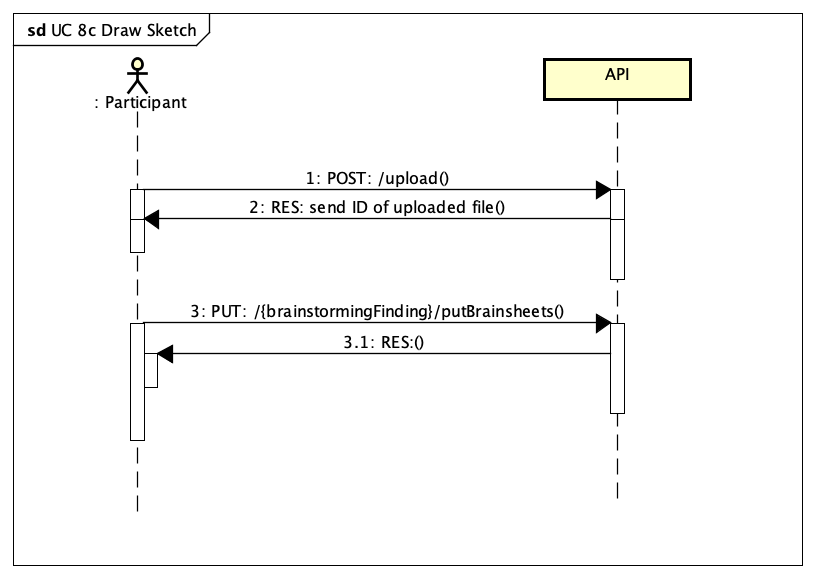
\includegraphics[width=1\linewidth]{img/anforderungen/Seq-Draw-Sketch}
	\caption[Ablauf beim Skizzieren]{Ablauf beim Skizzieren}
	\label{fig:Seq-Draw-Sketch}
\end{figure}

\begin{basedescript}{
		\desclabelstyle{\multilinelabel}
		\desclabelwidth{4.5cm}
		\setlength{\itemsep}{5ex}}	
	\item[\textit{UC8e Insert Pattern:}] Nachdem eine Brainwave gestartet ist (siehe 12 in Abbildung \ref{fig:Seq-Methode635}) und sich der Participant dazu entschlossen hat, ein Pattern als Idee zu nutzen, klickt er auf das Plus-Zeichen neben der Texteingabe und wählt das Pattern als Ideentyp aus. Nun wird ein GET-Request an das API gesendet, was als Antwort eine Liste aller verfügbaren Patterns zur Folge hat. Der Participant kann nun das gewünschte Pattern auswählen.
	Auch hier wird nun wieder, wie bis anhin (siehe 12.1 in Abbildung \ref{fig:Seq-Methode635}), das gesamte Brainsheet, welches nun auch das Pattern in der entsprechenden PatternIdee gespeichert hat, an die API geschickt.
\end{basedescript}

\begin{figure}[h]
	\centering
	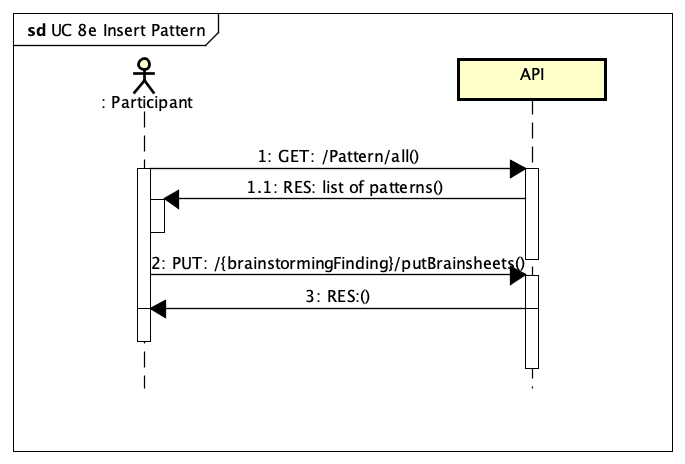
\includegraphics[width=1\linewidth]{img/anforderungen/Seq-Insert-Pattern}
	\caption[Ablauf beim Einfügen eines Patterns]{Ablauf beim Einfügen eines Patterns}
	\label{fig:Seq-Insert-Pattern}
\end{figure}

\newpage
\subsubsection{Nicht-Funktionale Anforderungen}
Wie schon in unserer Studienarbeit halten wir uns auch hier wieder an die Standards ISO 9126\cite{ISO9126} bzw. dessen Nachfolger ISO 25010\cite{ISO9126_ISO25010}, welcher Gegensatz zum Standard ISO 9126 noch ausführlicher ist. Beide ISO-Normen liefern daher eine gute Checkliste für jegliche Art von Systemanforderungen.

\begin{figure}[h]
	\centering
	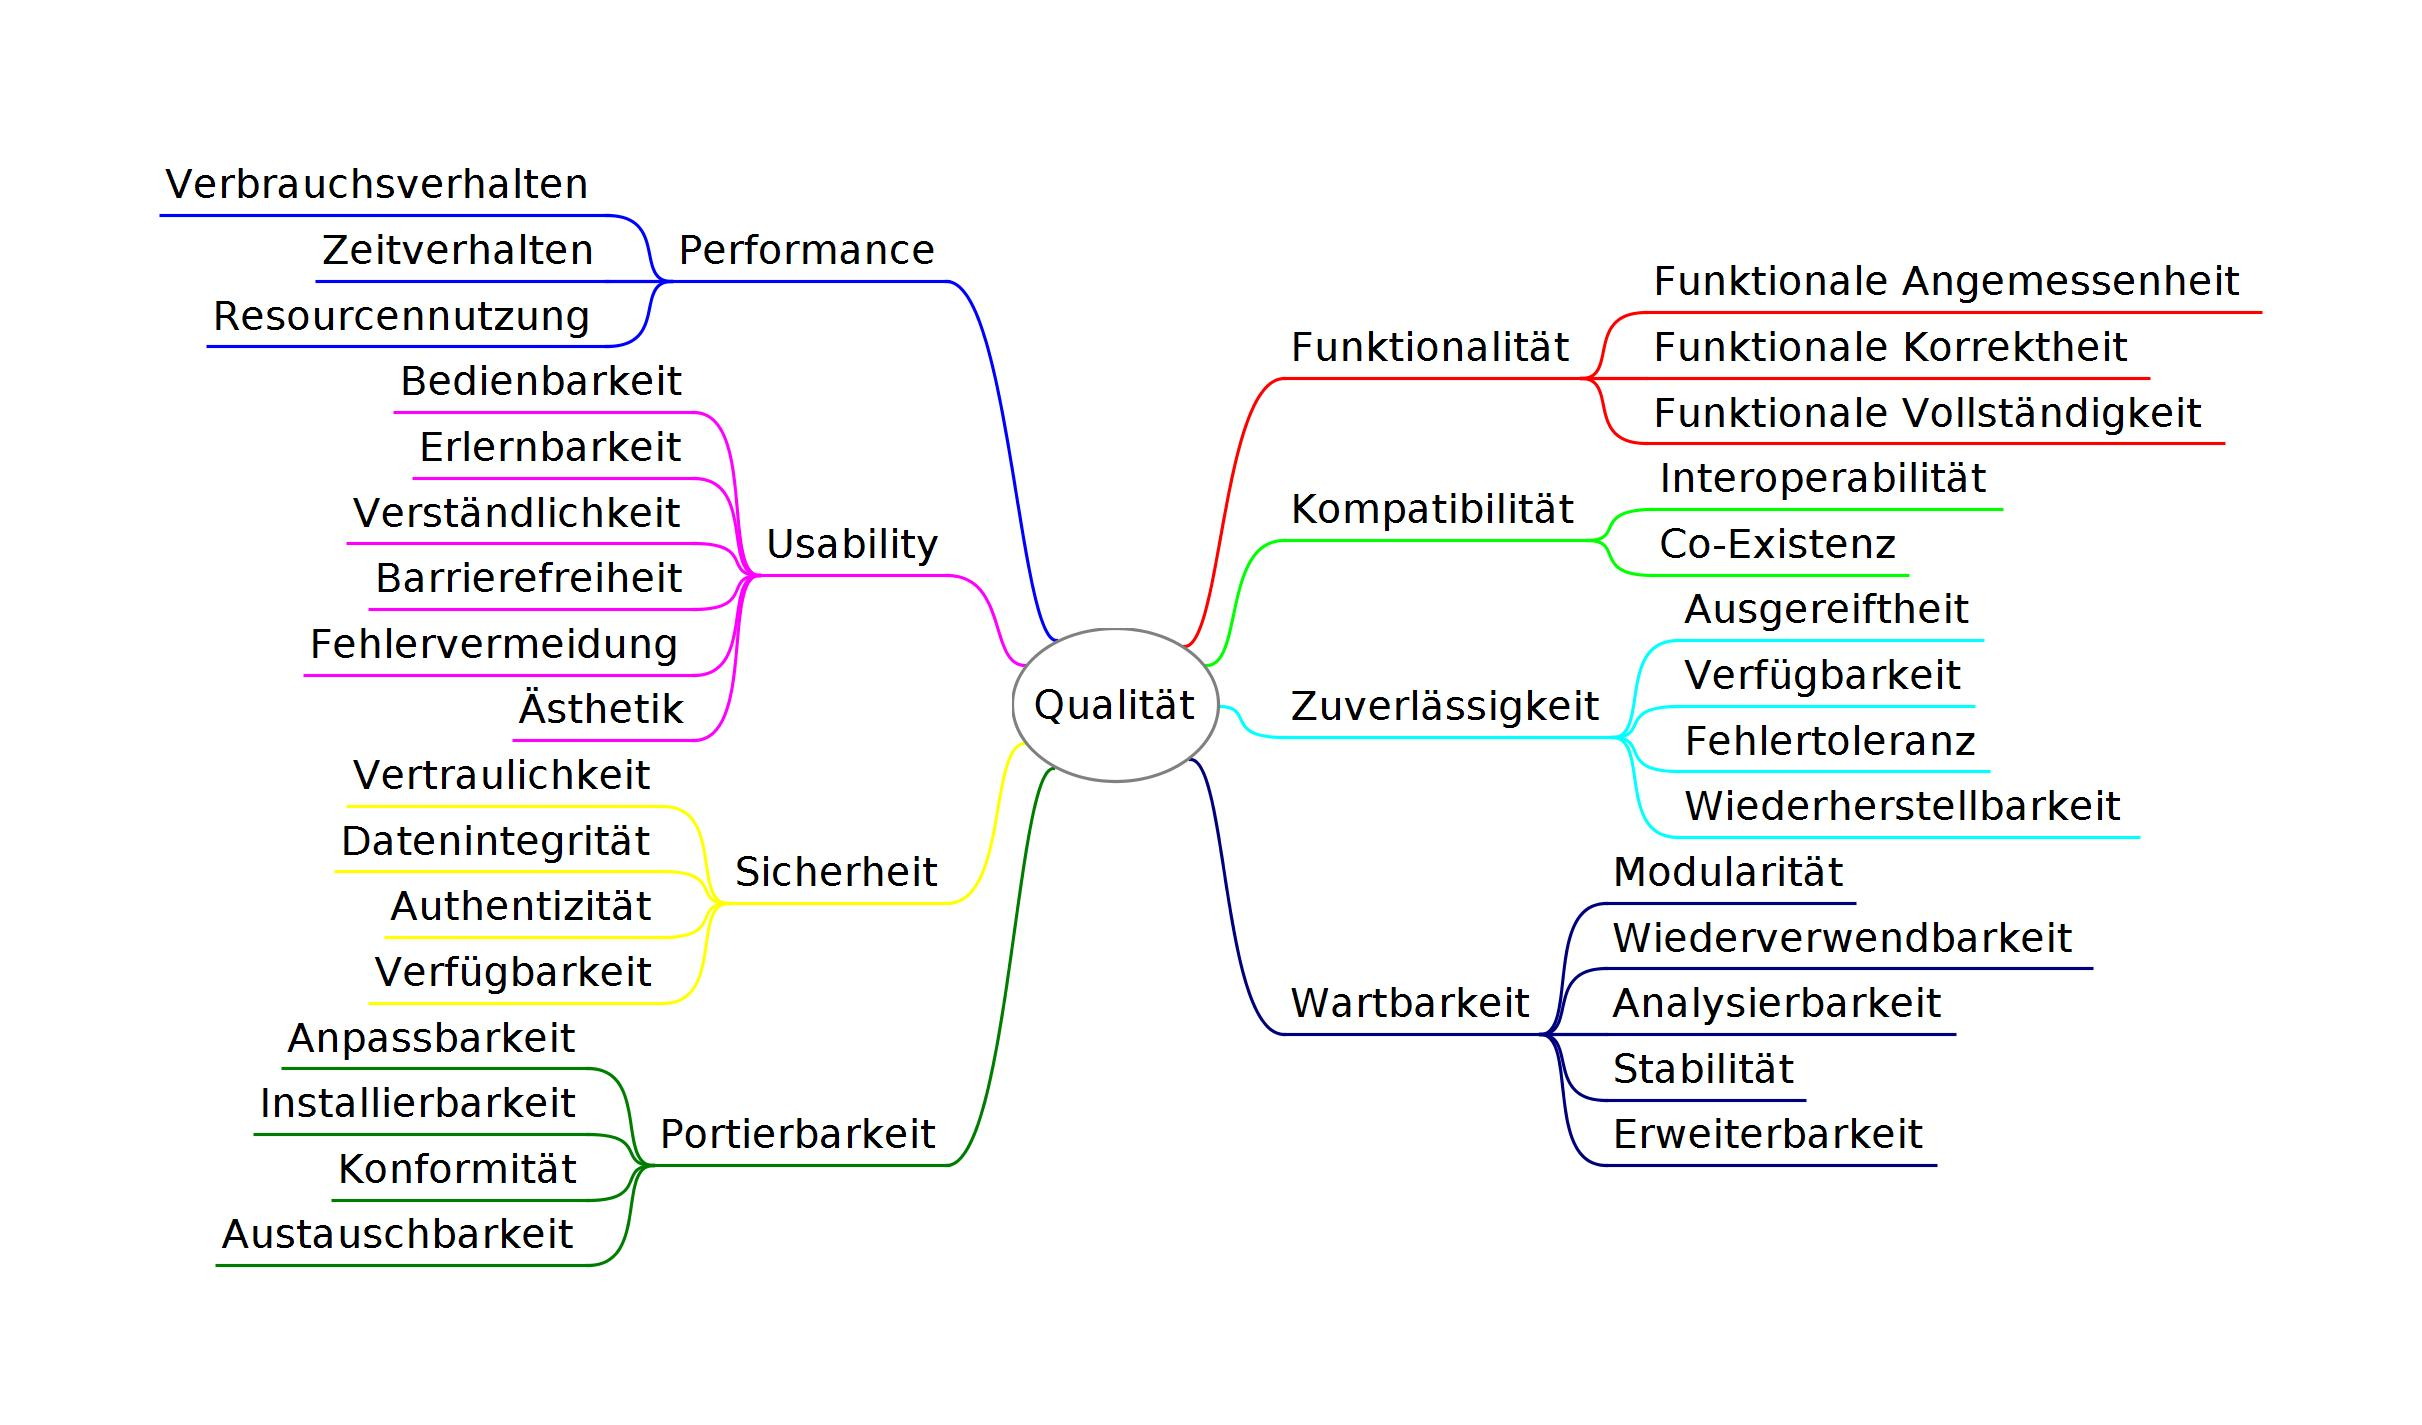
\includegraphics[width=1\linewidth]{img/anforderungen/quality}
	\caption[Anforderungskategorien nach ISO 25010]{Anforderungskategorien nach  ISO 25010}\cite{ISO25010_Bild}
	\label{fig:ISO 25010}
\end{figure}

Im Gegensatz zur Studienarbeit wollen wir uns bei dieser Arbeit aber vor allem auf Faktoren wie Erweiterbarkeit und Modularität konzentrieren. Auch sollen Faktoren wie Zeitverhalten und Ästhetik stärker in den Vordergrund rücken. 

Die bekannten nicht-funktionale Anforderungen aus der Studienarbeit bleiben allerdings weiter bestehen. Um genaue und erfüllbare nicht-funktionale Anforderungen zu definieren, müssen die SMART-Kriterien \cite{SMART} erfüllt sein.

Um die SMART-Kriterien noch besser zu erfüllen, haben wir uns in dieser Arbeit dazu entschieden, sogenannte Landing Zones (gemäss HSR-Vorlesung: Application Architecture vom 25.09.2018) zu definieren. Diese erlauben es flexibler auf Ziele einzugehen und Toleranzen für akzeptable Werte festzusetzen.

\begin{center}
    \begin{tabular}{ | p{6cm} | p{2.5cm} | p{2.5cm} | p{2.5cm} |}
    	\hline
    Kriterium & Minimum & Optimal & Übertroffen \\ 
    	\hline
    \textbf{Zeitverhalten} \newline Zeitkritische Kommunikation (Abgabe von Ideen/Brainsheets) zwischen Server und App beträgt & 2 Sekunden & 1 Sekunden & weniger als 1 Sekunde \\
    	\hline
    \textbf{Erweiterbarkeit} \newline Die Anzahl an neuen Ideenarten, welche mit der bestehenden Architektur als umsetzbar gelten, wird als ... angesehen & zu wenig (0-1) & ausreichend (1-5) & unbegrenzt ($>$5)\\
    	\hline
    \textbf{Modularität} \newline Die App ist innert ... Tagen um eine neue Ideenart erweitert & 5 Tage & 2 Tage & weniger als 1 Tag \\
    	\hline
    \textbf{Ästhetik} \newline Die Anziehungskraft gegenüber dem Endnutzer wird als ... charakterisiert & ausreichend für eine kritische Masse an Nutzern & nachhaltig & tägliche Nutzung in kritischen Projekten \\
    	\hline
    \textbf{Ausgereiftheit} \newline Der Grad der Ausgereiftheit oder Reife wird als ... angesehen & ungenügend für den produktiven Einsatz (Prototypen-Stadium) & genügend für den produktiven Einsatz, kann aber immer noch in Fehlerzustände gelangen & kaum Fehlerzustände und somit keine Abstürze der App  \\
    	\hline
    \end{tabular}
\end{center}
